\chapter{Introduction}
\label{chp:chp1}

Our brain is our most precious yet most mysterious organ. It consists
of nearly 100 billion neurons, of which typically has 10,000
connections that extend up to a meter. As such, it is an intricate web
that enable us to experience the world. In addition to neurons, the
brain consists of about the same number of glial cells, around 700
kilometers of blood vessels, the extracellular matrix, and is
surrounded by clear water-like cerebrospinal fluid, which together all
work to maintain the delicate neurons' environment in a healthy
state. At the whole-organ level, this is already incredibly complex,
yet this is only part of the story; at any given time, various
processes are happening in the brain, such as the electrical impulses
between neurons and the complex chemical signaling that helps to
maintain homeostasis. Due to the innate micro-scale complexity of the
brain, a natural approach, in attempting to understand the brain's
physiology and function, is offered by homogenized, continuum-based
modeling; here, the focus is on modeling the large-scale behavior
arising from the aggregate of small-scale contributions.

While continuum-based brain modeling has many applications, our
motivation for writing this book and the corresponding software tools
comes from recent theories concerning the restorative mechanisms of
sleep. Recent theories consider the brain a porous and elastic
(poroelastic) medium, where the elastic medium consists of the cells,
and the fluid-filled pores are the extra-cellular matrix (of course,
hyperelastic and viscoelastic materials~\cite{goriely2015mechanics,
  budday2019fifty} could also be considered). In this setting, a
paradigm shift was introduced by the glymphatic theory, proposed and
developed over the last eight years by the Nedergaard
group~\cite{iliff2012paravascular}. The glymphatic theory proposes
that extra-cellular diffusion, as described in the seminal work of
Sykov{\'a} and Nicholson~\cite{sykova2008diffusion}, is not sufficient
to explain the fundamental transport processes in the brain. In
particular, pressure-driven convective flow is hypothesized to wash
away the larger molecules of the metabolic waste products produced
during the day~\cite{iliff2012paravascular, jessen2015glymphatic,
  xie2013sleep}. Such metabolic waste proteins are observed to
accumulate in patients with neurodegenerative diseases such as
Alzheimer's or Parkinson's disease.

This topic has received a great deal of attention from the modeling
community when it comes to the mechanisms at the microscopic level,
e.g.~\cite{aldea2019cerebrovascular, daversin2020mechanisms,
  diem2017arterial, holter2017interstitial, ray2019analysis,
  sharp2019dispersion, smith2017test}. However, very few works address
the macroscopic level and how to employ modeling in a patient-specific
manner, see e.g.,~\cite{chou2016fully, lee2019mixed}. Mesh generation
based on medical images, typically integrating images of different
types, plays a critical role in achieving a patient-specific
assessment. Our intention with this book is to equip the reader with
software tools to perform studies of this kind.

Many other applications involve continuum-based models of the brain's
physiology.  For instance, alternative macroscopic theories involving
the prion-related development of Alzheimer's disease have been
proposed~\cite{fornari2019prion, kevrekidis2020anisotropic}. Another
interesting observation is that astronauts often experience visual
impairments and are at risk of developing early dementia as a
consequence of their periods in low or zero gravity. This seems to be
a result of intracranial pressure changes and a shift in fluid volumes
in intracranial compartments~\cite{alperin2018spaceflight}.  Another
well-known computational modeling problem relates to epilepsy:
specifically, the inverse problem of electroencephalography (EEG) in
determining the source of an epileptic seizure via an elliptic
PDE~\cite{grech2008review}.

\begin{figure}
  \begin{center}
  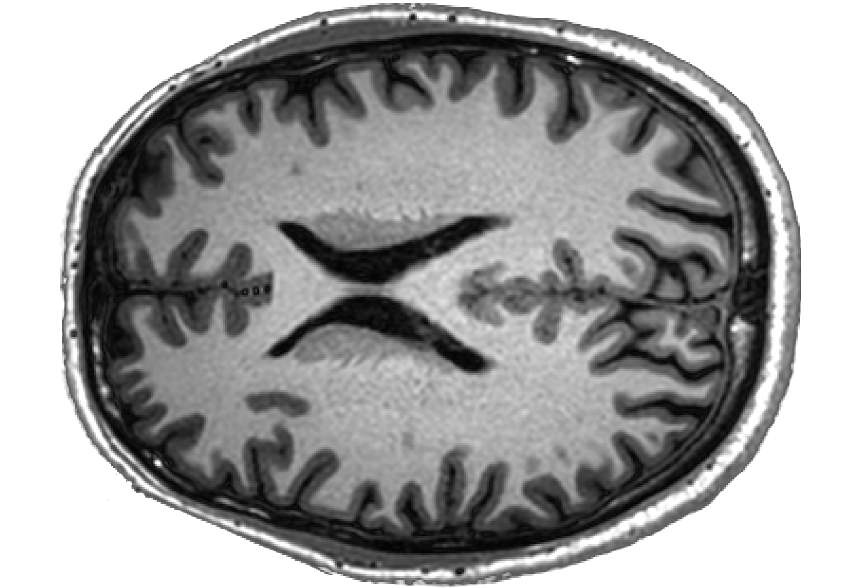
\includegraphics[height=2.3cm]{./graphics/chp1/T1-image-rot-white}
  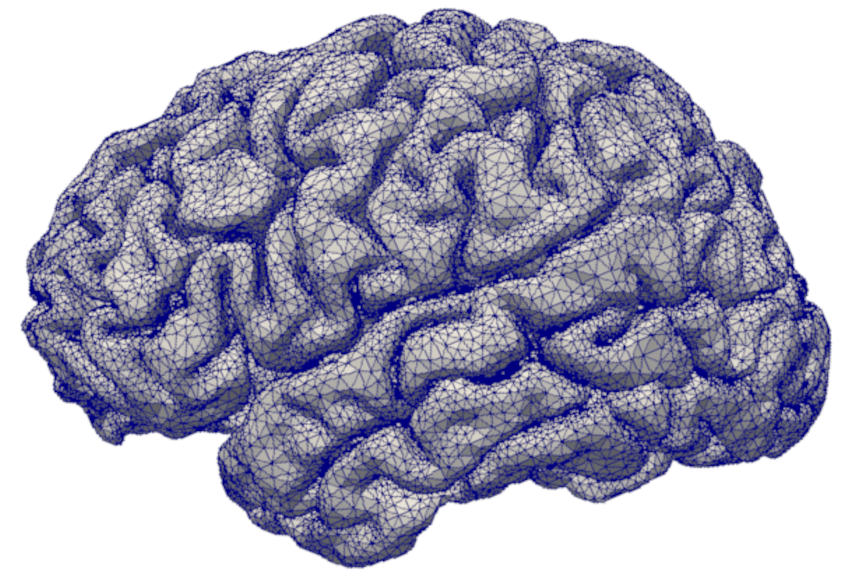
\includegraphics[height=2.3cm]{./graphics/chp1/ernie-volume-64}
  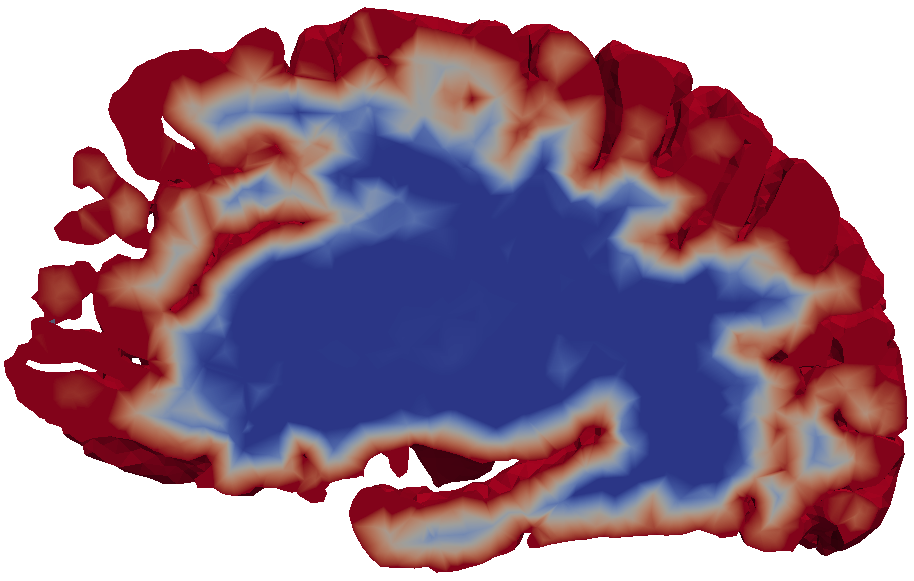
\includegraphics[height=2.3cm]{./graphics/chp1/soltn-t30-crop}
  \hfill
  \end{center}
  \caption{Going from magnetic resonance (MR) images of a human brain
    to a numerical simulation of a biophysical phenomenon. From left
    to right: (a) An MR image of a human brain viewed along the axial
    direction, (b) a finite element mesh extracted from the MR image,
    (c) a snapshot of a tracer distribution simulation over this
    mesh. MR image types are discussed in Chapter~\ref{chp:chp2}.}
  \label{fig:chp1:pipeline}
\end{figure}

This book provides the computational resources that form the
foundations of continuum-based modeling of the human brain. Although
we don't focus explicitly on the exciting multiphysics applications
mentioned above, the approach discussed here is generalizable to
multiphysics problems. You, the reader, will learn how to formulate,
set-up and implement mathematical and computational models of brain
biophysics in patient-specific geometries using finite element
simulations and MR images (see Figure \ref{fig:chp1:pipeline}). We
will use the evolution and distribution of a solute concentration due
to diffusion as a model problem, and increase the complexity of the
data and techniques involved over the course of the book. Of course,
the process involves several challenges and pitfalls, which will be
outlined.

\section{A model problem}

\index{diffusion equation} Suppose that we aim to study the diffusion
of a solute concentration in a region of the brain. The region
$\Omega$ could represent the left brain hemisphere or a smaller region
such as the hippocampus, while the concentration $u$ could represent
an injected tracer used in imaging (such as
gadobutrol~\cite{ringstad2018brain} or
dextran~\cite{iliff2013cerebral}) or possibly a metabolic waste
protein, such as amyloid-$\beta$ or tau. We can describe this model
problem by a time-dependent partial differential equation (PDE): find
the concentration $u = u(t, x)$ at spatial points $x \in \Omega$ and
time points $t > 0$ such that
\begin{subequations}
  \label{eq:diffusion}
  \begin{align}
    \label{eq:diffusion:a}
    u_t - \Div D \Grad u &= f &&\text{ in } (0, T] \times \Omega, \\
    \label{eq:diffusion:b}
    u &= u_d && \text{ on } (0, T] \times \partial \Omega, \\
    \label{eq:diffusion:c}
    u(0, \cdot) &= u_0 && \text{ in } \Omega.
  \end{align}
\end{subequations}
In the diffusion equation~\eqref{eq:diffusion:a}, $u$ is the unknown
field, while $D$ is the diffusion tensor coefficient and $f$
represents any source or sink for the concentration within the
domain. The subscript $t$ denotes the time derivative, $\Div$
represents the divergence and $\Grad$ the spatial gradient. The second
equation~\eqref{eq:diffusion:b} gives a boundary condition: the
function $u_d$ represents a known distribution of the concentration on
the boundary $\partial \Omega$ for all times. The third
equation~\eqref{eq:diffusion:c} gives an initial condition for the
solute concentration: the function $u_0$ represents the known initial
concentration distribution throughout $\Omega$ at $t=0$. The combined
problem \eqref{eq:diffusion} is a complete initial boundary-value
problem and will be our model problem.


\section{On reading this book}
This text does not assume that the reader is well versed in anatomy or
neuroscience.  In fact, most of the anatomical knowledge needed to
follow along with this text is covered in
Chapter~\ref{sec:chp2:anatomy}.  We have also made liberal use of
footnotes and citations to inform the reader of additional
interesting, or contextually useful, anatomical or physiological
details. This text does, however, assume a basic knowledge of
PDEs. For instance, the diffusion equation \eqref{eq:diffusion} is a
classical continuum-based PDE with well-known behavior in both the
mathematical and numerical sense. The reader unfamiliar with this
equation is advised to first consult an introductory text on solving
PDEs using the finite element
method~\cite{gockenbach2006understanding, langtangen2016solving,
  langtangen2019introduction,tveito2004introduction}.

The reader is assumed to be comfortable executing commands from a
command line in a terminal window (also canonically referred
to as a command window or command prompt). Terminal commands
will be formatted throughout as:
\terminal{\$ cd ..}
\noindent Commands at the operating-system (OS) level, such as that above,
can differ from OS to OS, and we mainly demonstrate Linux commands
here.

We also assume the reader is familiar with the fundamentals of the
Python programming language or, alternatively, can understand the
syntax well enough to follow the source code that appears throughout;
we will not use any advanced Python programming techniques. We use
Python 3 throughout, so please ensure that you have Python version 3.0
or any later version installed. You can check your Python version with
either of the following terminal commands:
\terminal{\$ python {\ddash}version \\
\$ python3 {\ddash}version
}

We will use the Python interface to the FEniCS Project finite
element software~\cite{alnaes2015fenics}, and we assume that the
reader is familiar with the material covered by the FEniCS
tutorial~\cite{langtangen2016solving}.

\section{Datasets and scripts}

\index{mri2fem datasets and scripts}

The datasets and scripts used and described in this book are openly
available and associated with its Zenodo community: \\
\url{https://zenodo.org/communities/mri2fem/}. 
\begin{itemize}
\item
  The book dataset, including MR images, can be downloaded from \\
  \url{http://doi.org/10.5281/zenodo.4386986}~\cite{kent_andre_mardal_2020_4386986}.
\item
  The book scripts can be downloaded from \\
  \url{http://doi.org/10.5281/zenodo.4386998}~\cite{kent_andre_mardal_2020_4386998}.
\item 
  A git repository containing the book and its scripts can be found 
  at: \\ \url{https://github.com/kent-and/mri2fem}.
\end{itemize}
We highly recommend that you download and unpack these materials
before reading further. We expect to update the Zenodo community with
script updates, updated installation guides and further material as
needed.
 
\section{Other software}
We will use a number of external tools in this book. Most of these
tools are available for several operating systems, with separate
installation instructions and dependencies for each system. For the
key external tools, we provide installation instructions for Linux
Ubuntu (version 20.04, but earlier or later versions should also work
along the same, or similar, lines). Whenever we refer to an Ubuntu-specific 
terminal command, we format it as follows:
\ubuntu{\$ sudo apt-get install ... }
\noindent We note that, before installing packages, it can be important to update
the Ubuntu package list. This can be done by the following command:
\ubuntu{\$ sudo apt-get update}
\noindent For other operating systems, we refer to the specific
software documentation for installation instructions.

\section{Book outline}

Chapter 2 provides an introduction to brain physiology and imaging, as
and outlines the software ecosystem that will take us from MR images
to numerical simulation. In Chapter~\ref{chp:chp3}, our aim is to get
up and running quickly: we step through the entire pipeline from
generating a volume mesh from MR image data to solving our model
problem~\eqref{eq:diffusion} on this mesh. In Chapter~\ref{chp:chp4},
we cover other aspects of meshing, including distinguishing between
gray and white matter, merging left and right hemispheres, and adding
parcellation labels. In Chapter~\ref{chap:dti}, we focus on diffusion
tensor imaging (DTI) and demonstrate how we can convert DTI data to a
numerical tensor field. Finally, Chapter~\ref{chp:chp6} brings
together everything from Chapters~\ref{chp:chp3} to \ref{chap:dti} to
present a realistic simulation of anisotropic diffusion in
heterogeneous brain regions.
 
